\documentclass[10pt, compress]{beamer}

\usetheme{metropolis}

\usepackage{booktabs}
\usepackage[scale=2]{ccicons}

\usepackage{amsmath}

%Icons
\usepackage{fontawesome}

%Syntax highlight
\usepackage{listings,xcolor}
\usepackage{inconsolata}

\definecolor{dkgreen}{rgb}{0,.6,0}
\definecolor{dkblue}{rgb}{0,0,.6}
\definecolor{dkyellow}{cmyk}{0,0,.8,.3}

% Language: PHP
\lstset{
  language        = php,
  basicstyle      = \small\ttfamily,
  keywordstyle    = \color{dkblue},
  stringstyle     = \color{red},
  identifierstyle = \color{dkgreen},
  commentstyle    = \color{gray},
  emph            =[1]{php},
  emphstyle       =[1]\color{black},
  emph            =[2]{if,and,or,else},
  emphstyle       =[2]\color{dkyellow}
}

%\usepgfplotslibrary{dateplot}


\title{Unauthenticated encryption in the wild}	
%\subtitle{}
\date{\today}
\author{Carl Svensson}
\institute{SEC-T 2017}

\begin{document}

\maketitle

\begin{frame}{About me}
  
	\begin{columns}
		\begin{column}{0.6\textwidth}  
  
  		\begin{itemize}
		  \item Carl Svensson, 26
		  \item MSc in Computer Science, KTH
		  \item Head of Security, Kry
		  \item CTF-player, HackingForSoju
		  \item \faEnvelope \hskip 2mm calle.svensson@zeta-two.com
		  \item \faTwitter \hskip 2mm  @zetatwo
		  \item \faGlobe \hskip 2mm https://zeta-two.com
		\end{itemize}
		
		\end{column}
		\begin{column}{0.4\textwidth} 
			\begin{center}
			
\includegraphics[width=0.4\textwidth]{images/kth.jpg}
			\end{center}
			\vspace{1cm}
			
\includegraphics[width=\textwidth]{images/kry_logo.png}
		\end{column}
	\end{columns}
  
\end{frame}

\begin{frame}{Cryptography in 30 seconds}

 \begin{itemize}
  \item Transform data
  \item Maths, a lot of it
  \item Many possible goals
    \begin{itemize}
  	\item Confidentiality (Hide)
  	\item Integrity (Verify)
  	\item Authentication (Identify)
  	\item Non-Repudiation (No take-backsies)
    \end{itemize}  
  \item Modularity
  \end{itemize}    

\end{frame}


\begin{frame}{AES - Very good, at one specific thing}
  \begin{columns}
    \begin{column}{0.5\textwidth}
      \begin{itemize}
        \item Block cipher
        \item Key
        \item Basic building block
        \item No known attacks*
      \end{itemize}
    \end{column}
    \begin{column}{0.5\textwidth}
      \\
      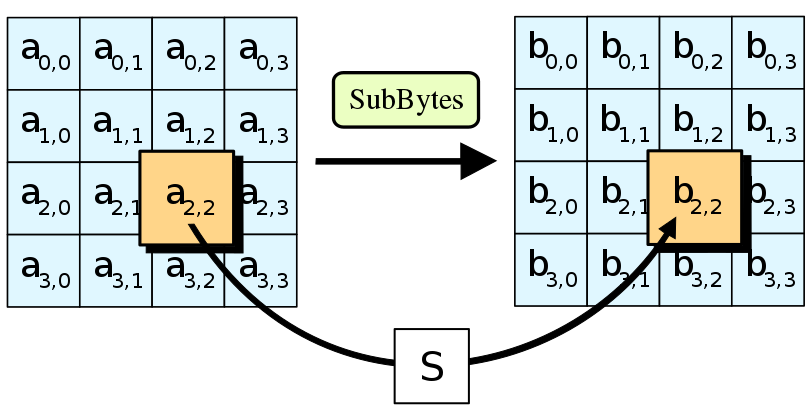
\includegraphics[width=0.65\textwidth]{images/aes-sub.png} \\
      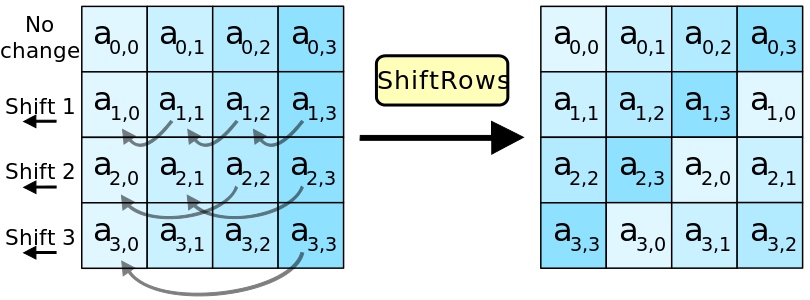
\includegraphics[width=0.65\textwidth]{images/aes-shift.png} \\
      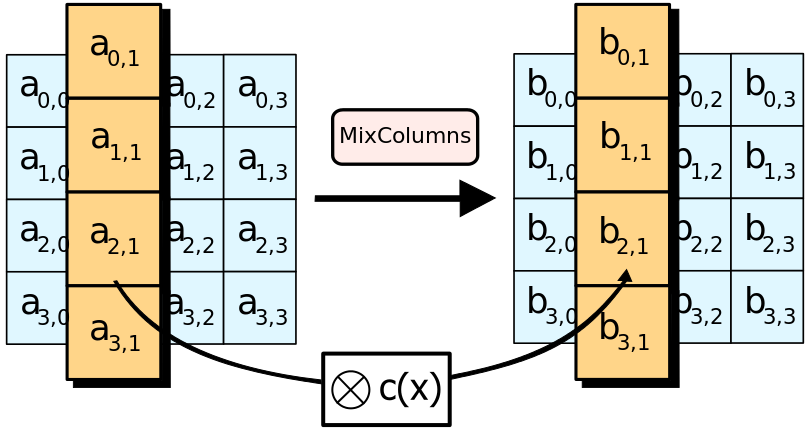
\includegraphics[width=0.65\textwidth]{images/aes-mixcolumns.png}\\
      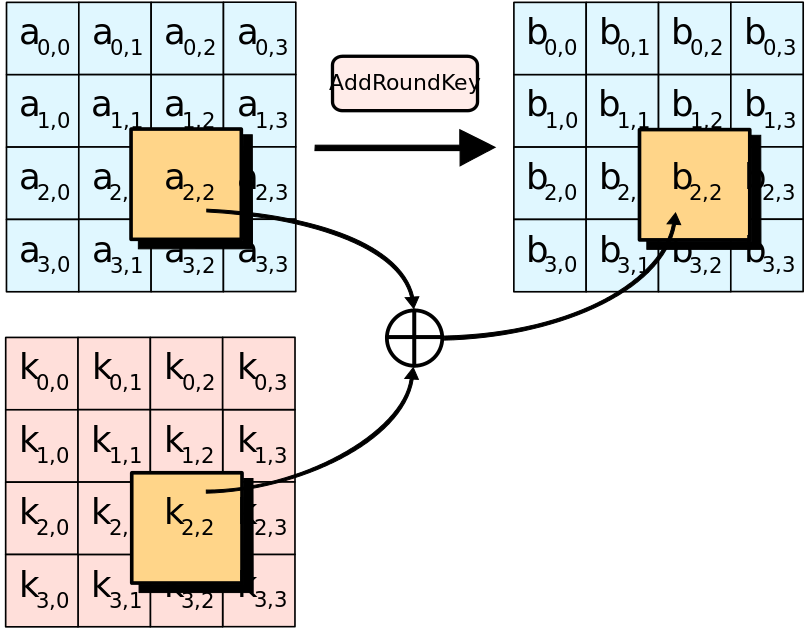
\includegraphics[width=0.65\textwidth]{images/aes-roundkey.png} \\
    \end{column}
  \end{columns}


\end{frame}
  
  
\begin{frame}{Block cipher modes, when you have more data}
  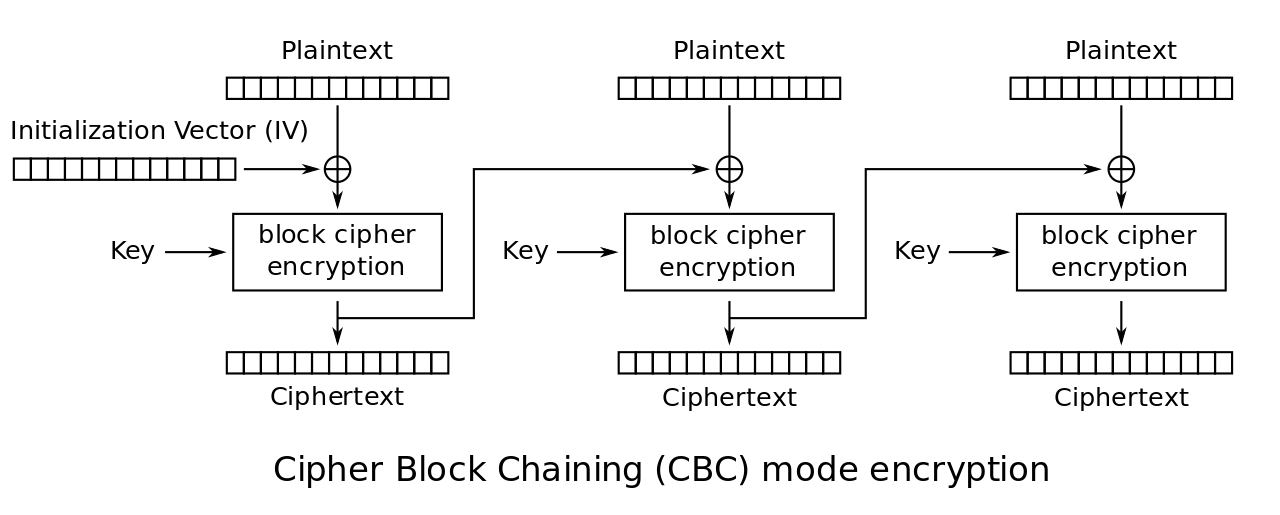
\includegraphics[width=0.9\textwidth]{images/1280px-CBC_encryption.svg.png} \\
  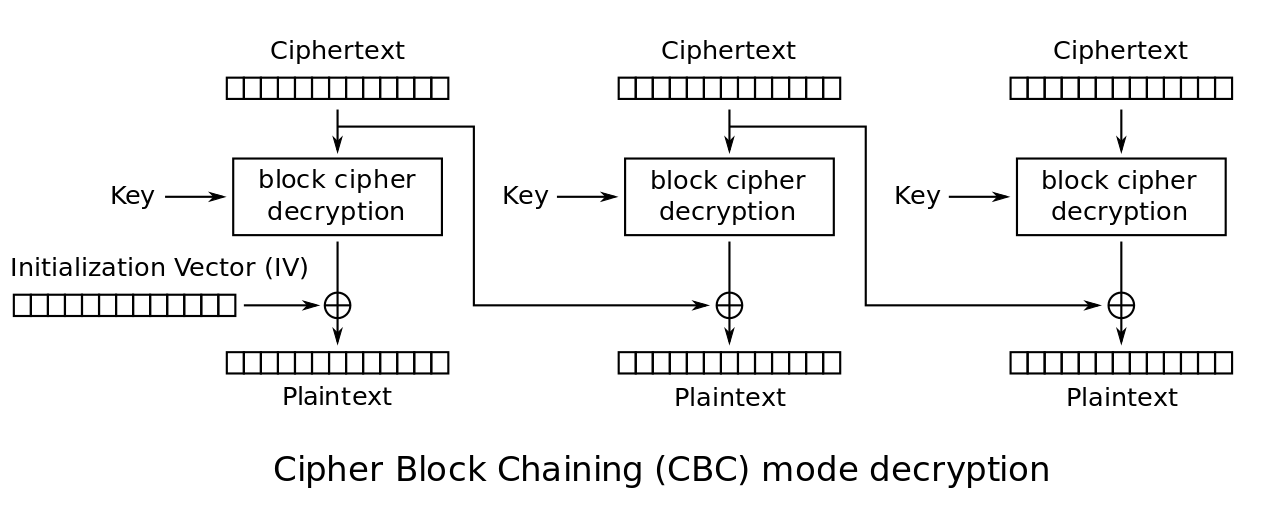
\includegraphics[width=0.9\textwidth]{images/1280px-CBC_decryption.svg.png} \\
\end{frame}


\begin{frame}{Encryption is not authentication}
\begin{columns}
    \begin{column}{0.5\textwidth}
      \begin{itemize}
        \item A priori, no way to differentiate
        \item Has to accept all ciphertexts
        \item Might be able to tell later
        \item The Cryptographic Doom Principle

      \end{itemize}
    \end{column}
    \begin{column}{0.5\textwidth}
      \\
      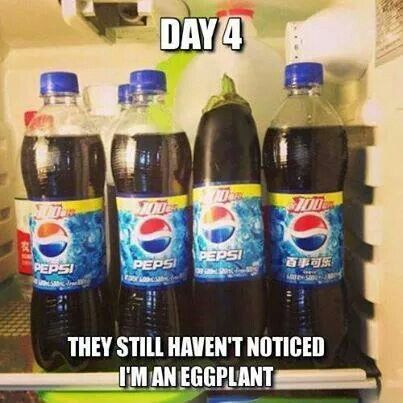
\includegraphics[width=\textwidth]{images/a8169e9a993e5cc8d3a06dd3e532791a--eggplants-so-funny.jpg} \\
    \end{column}
  \end{columns}
\end{frame}


\begin{frame}{Bit flipping attack}
  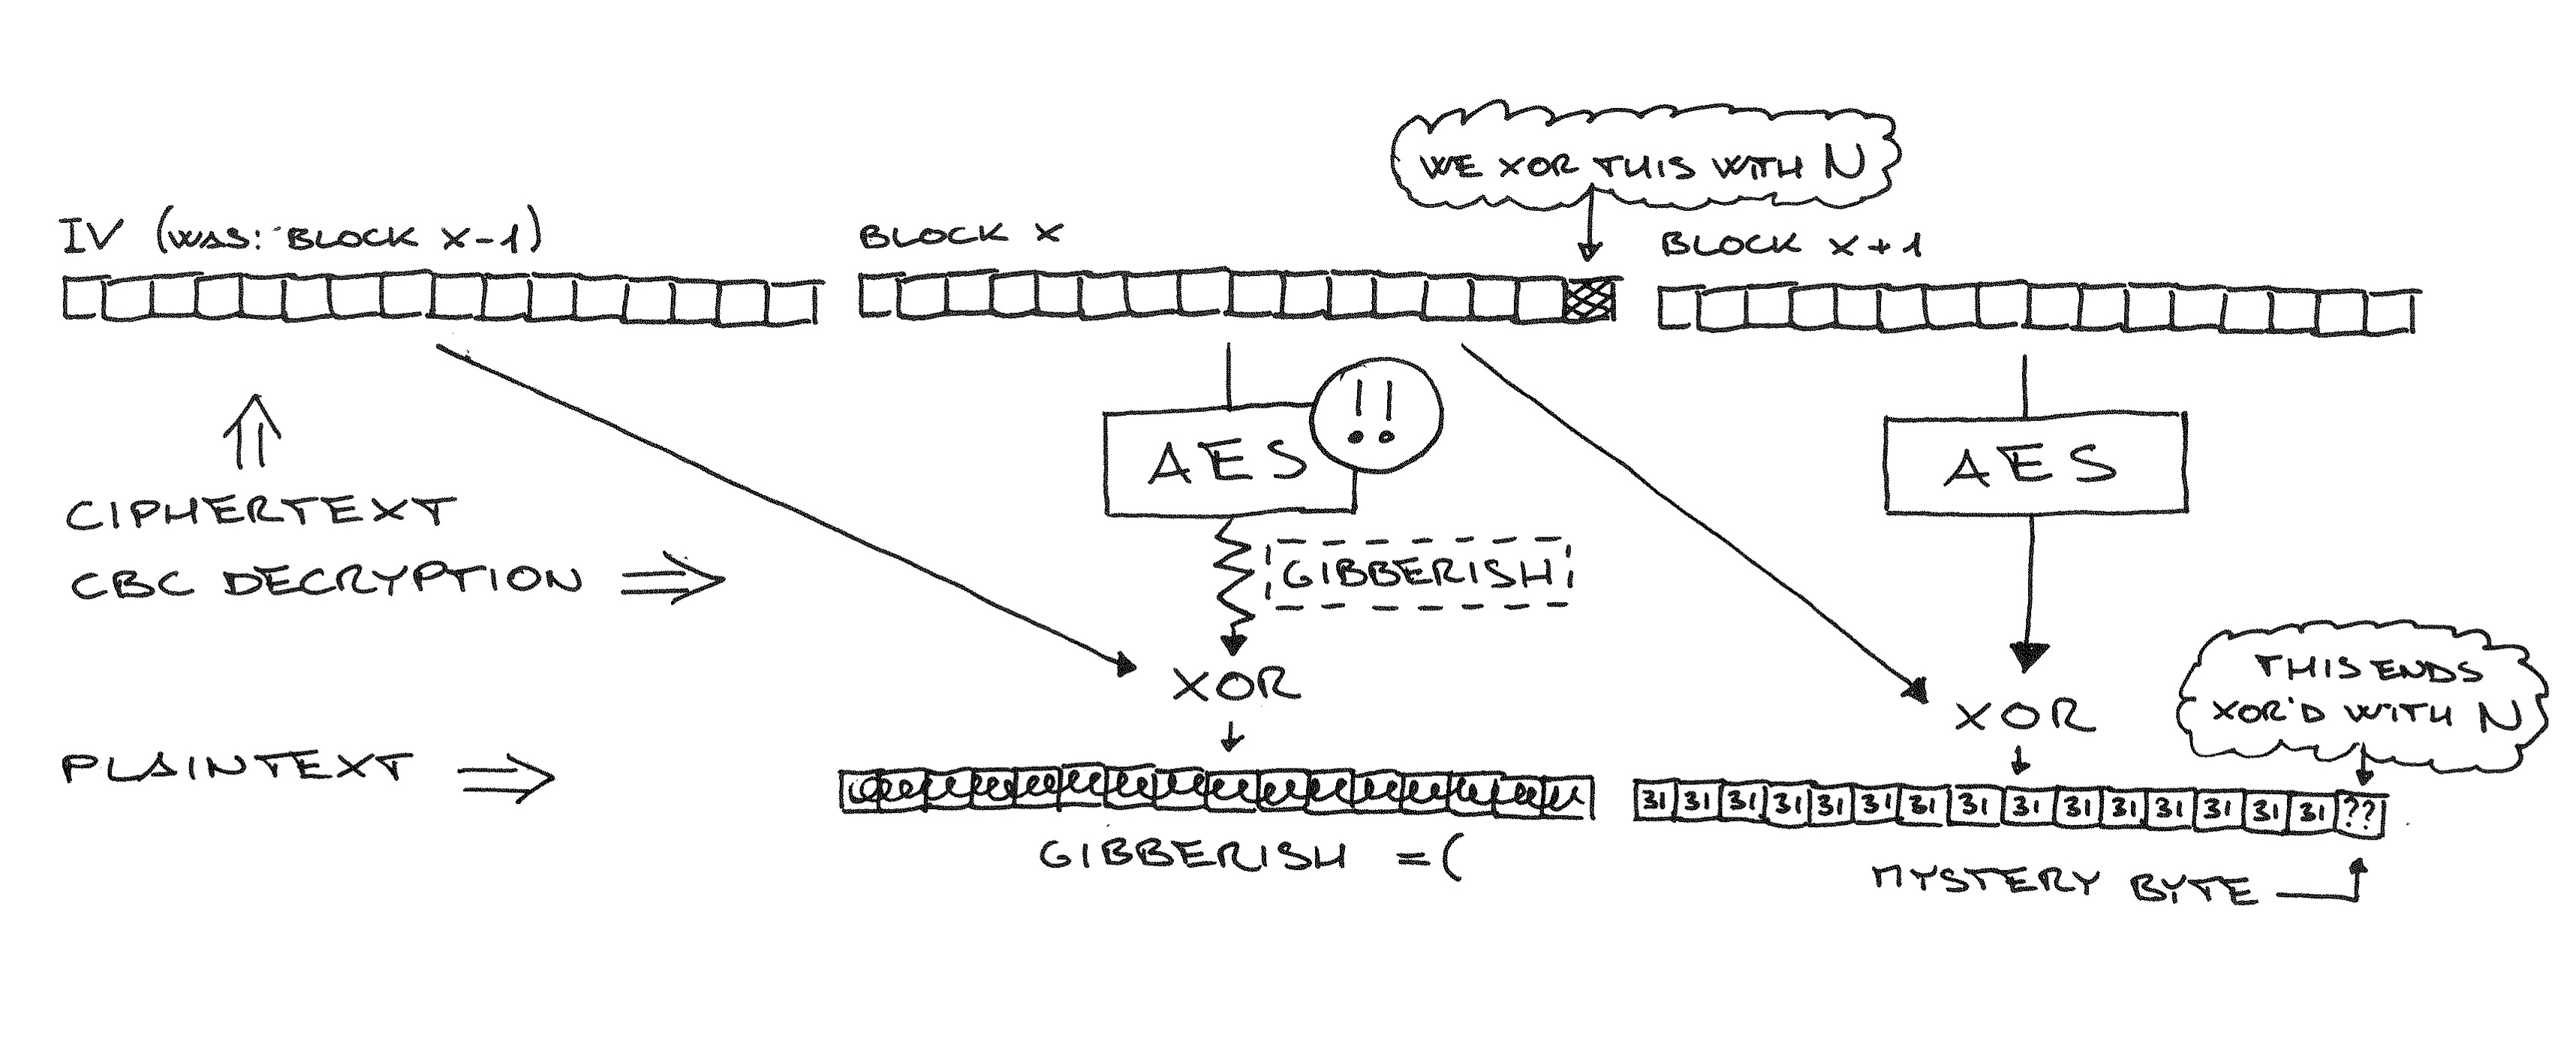
\includegraphics[width=\textwidth]{images/S22C-6e16050401360-1-1.jpg} \\
\end{frame}


\begin{frame}{Example: Open redirect as a service}
      \begin{itemize}
        \item https://link.a.com/AAAA/BBBBBBBBBBBBBBBBBBBBBB
        \item Known plaintext, just visit
        \item \( x \oplus m_1 = m_2 \Leftrightarrow x = m_1 \oplus m_2 \)
        \item Edit link contents
      \end{itemize}
      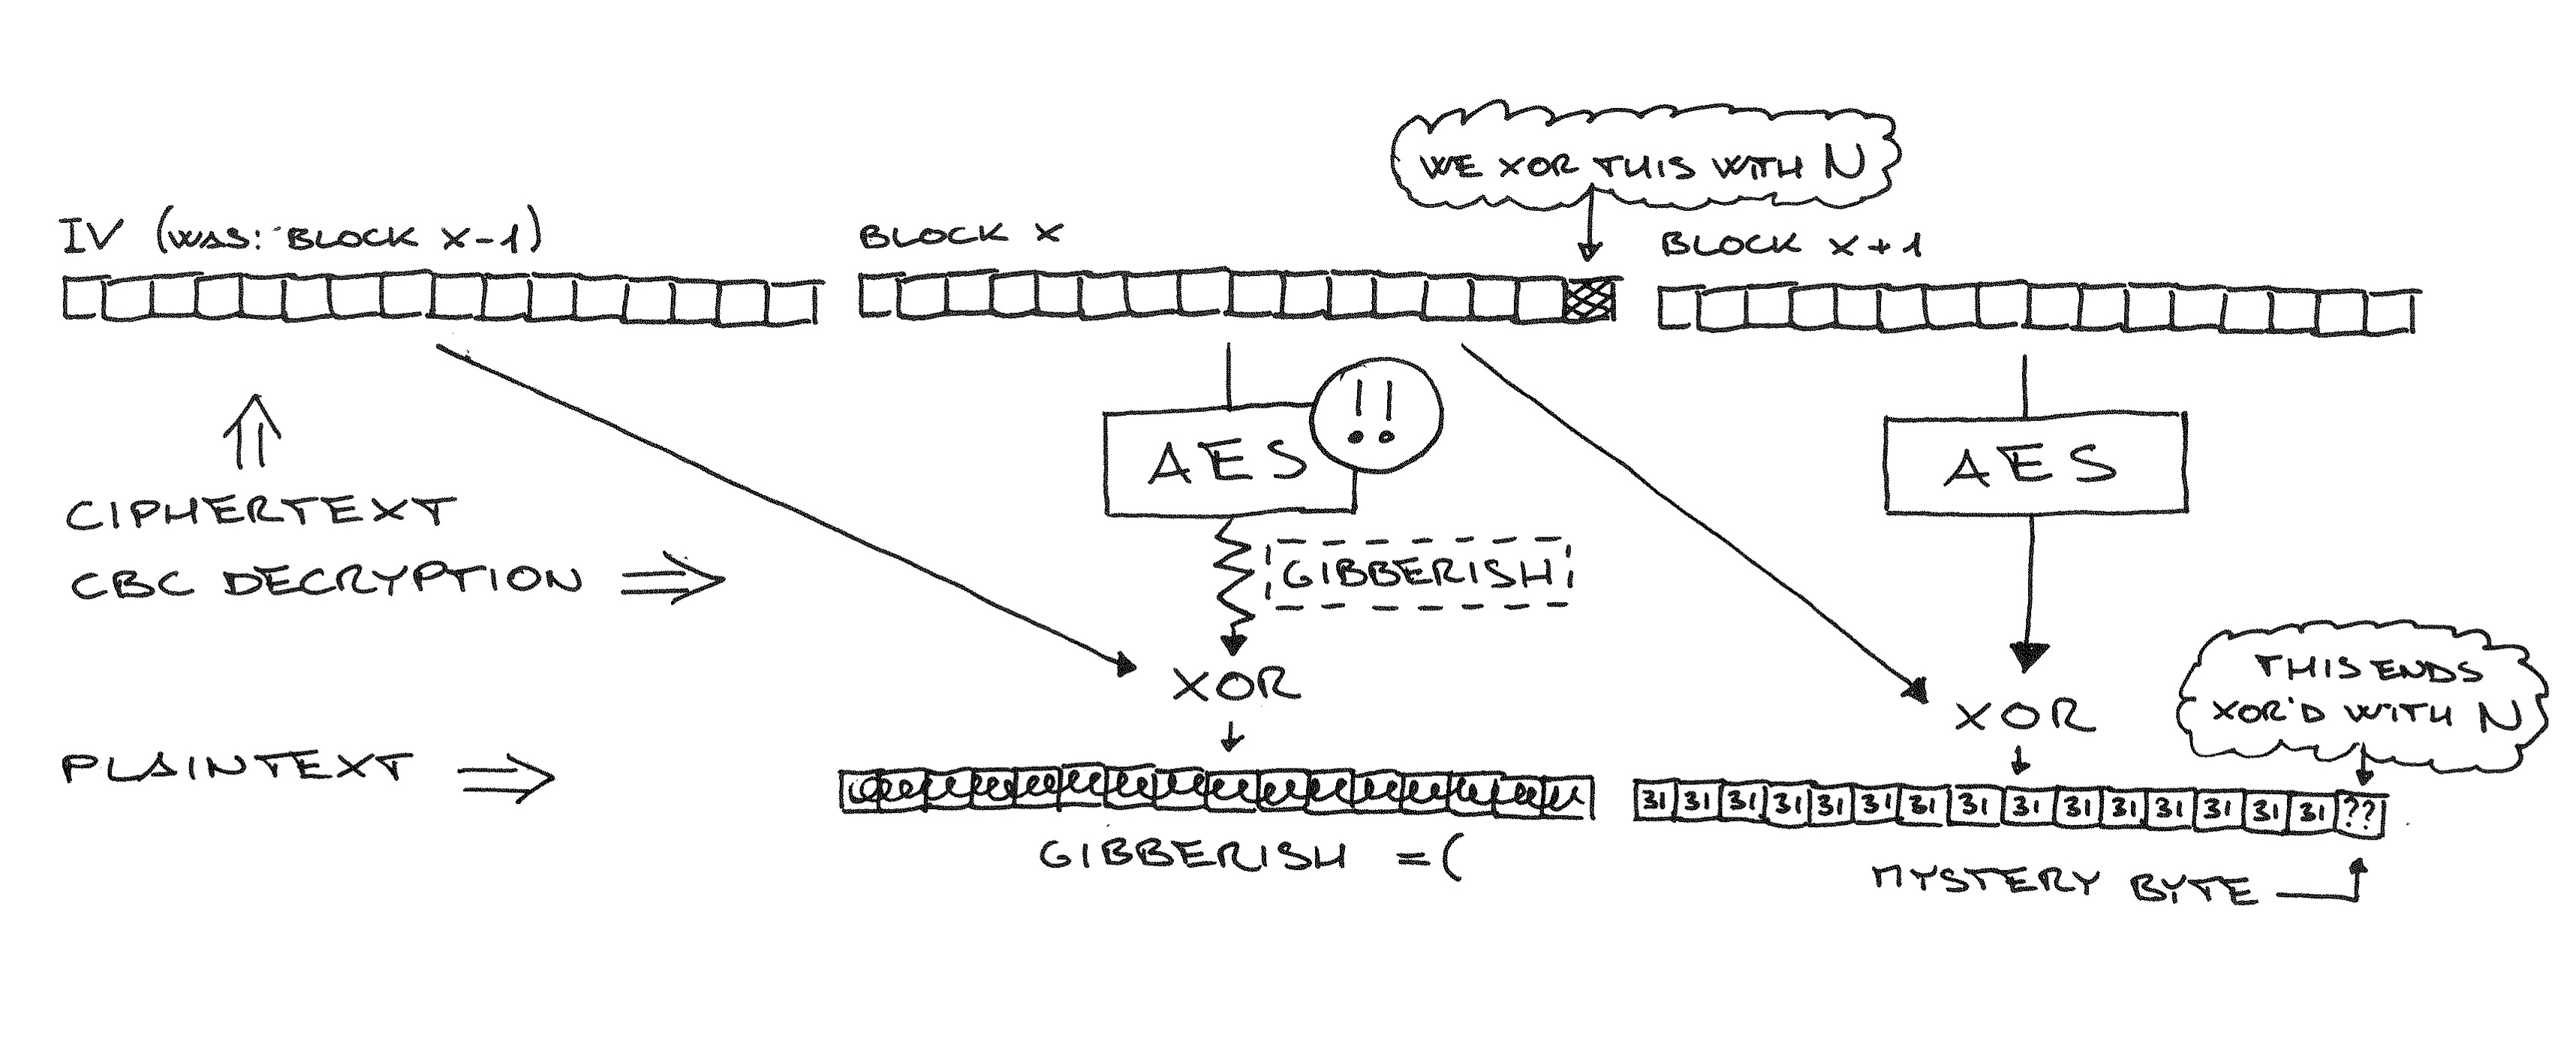
\includegraphics[width=\textwidth]{images/S22C-6e16050401360-1-1.jpg} \\
\end{frame}


\begin{frame}{Padding Oracle attack}
      \begin{itemize}
        \item PKCS7 padding
        \item bool oracle(input) \{ ... \} 
        \item Differing error messages
        \item \( x \oplus g = t \Leftrightarrow x = g \oplus t \)
        \item \( 16 \cdot 256 \ll 256^{16} \)
      \end{itemize}
    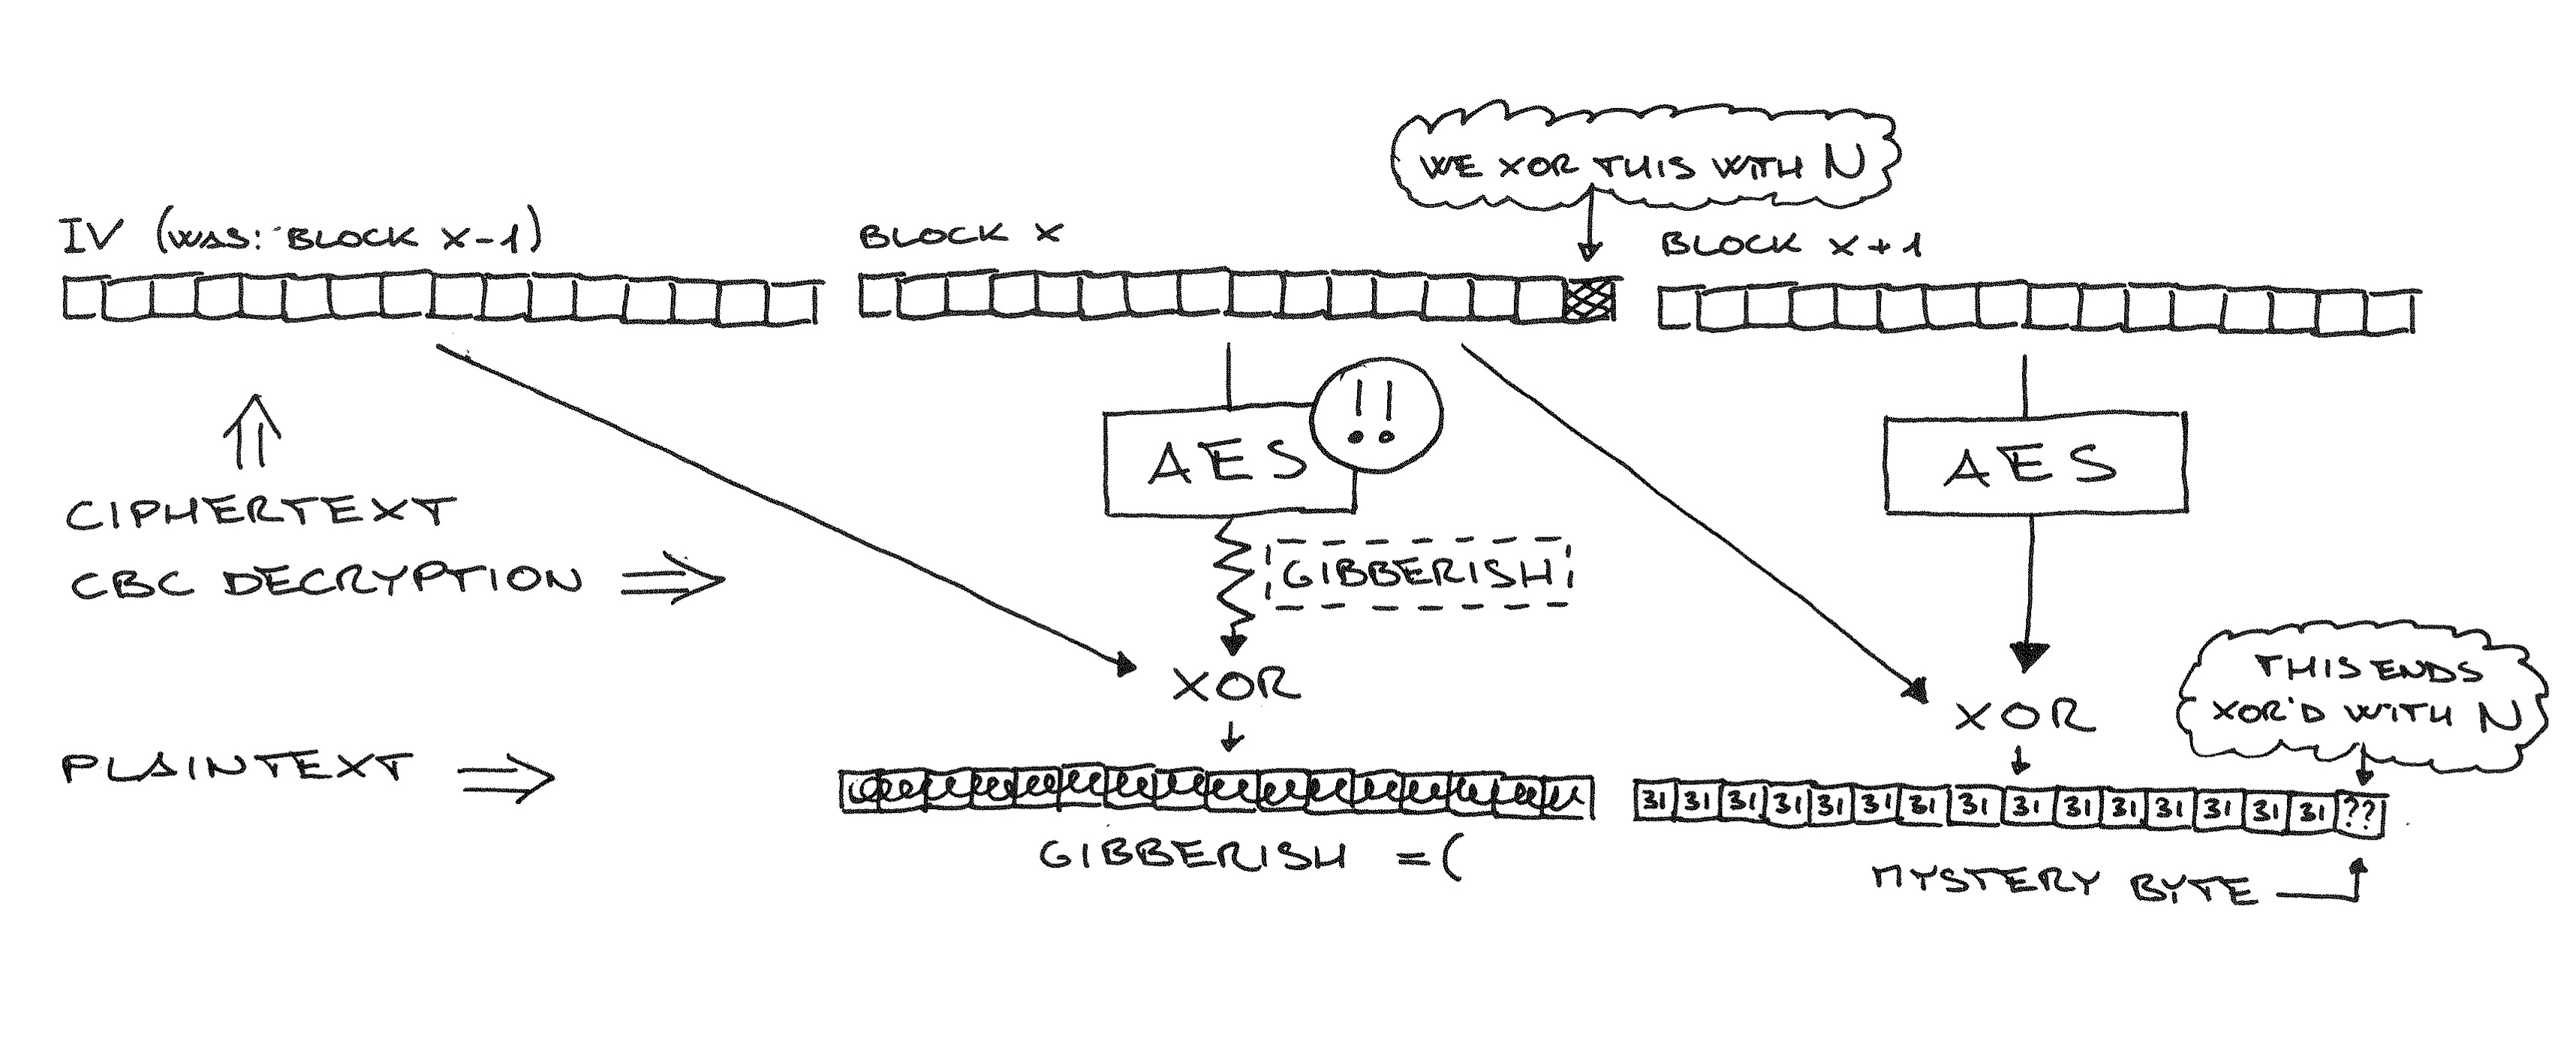
\includegraphics[width=\textwidth]{images/S22C-6e16050401360-1-1.jpg} \\
\end{frame}

\begin{frame}{Example: Extracting secrets -> RCE}
% File format [f_masterkey(key1)|f_key1(zipfile)]
% Padding oracle -> get key1
% Replace f_key1(zipfile)
% Arbitrary file write -> RCE
\begin{columns}
    \begin{column}{0.55\textwidth}
     \begin{itemize}
        \item Backup data
        \item File format: \( Enc_{Km}(key1)||Enc_{Ks}(zipfile) \)
        \item Padding Oracle -> Key -> Craft zip
        \item Zip relative paths -> RCE
      \end{itemize}
    \end{column}
    \begin{column}{0.45\textwidth}
      \\
      
\includegraphics[width=\textwidth]{images/WinZip_thumb.jpg} \\
    \end{column}
  \end{columns}



\end{frame}

\begin{frame}{What to do? Authenticate!}
\begin{itemize}
        \item Encryption AND authentication
        \item Message Authentication Code
        \item \( HMAC_k(message) = tag \)
        \item \( Verify_k(tag, message) \in {True, False} \)
      \end{itemize}
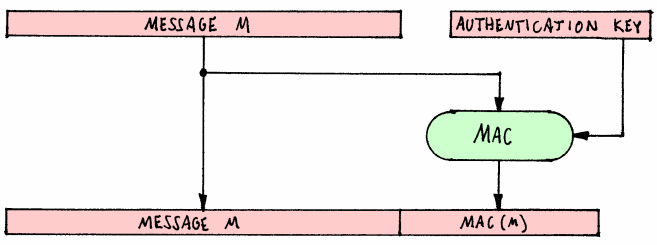
\includegraphics[width=\textwidth]{images/HashFig2.png} \\
\end{frame}


\begin{frame}[standout]
Thanks for listening!
\end{frame}



\end{document}
